%!TEX program = xelatex
\documentclass[dvipsnames, svgnames,a4paper,11pt]{article}
% ----------------------------------------------------
%   中山大学物理与天文学院本科实验报告模板
%   作者:Huanyu Shi,2019级
%   知乎:https://www.zhihu.com/people/za-ran-zhu-fu-liu-xing
%   Github:https://github.com/huanyushi/SYSU-SPA-Labreport-Template
%   Last update : 2023.4.10
% ----------------------------------------------------

% ----------------------------------------------------- 
%	加边框的命令
%	参考:https://tex.stackexchange.com/questions/531559/how-to-add-the-page-border-for-first-two-pages-in-latex
\usepackage{tikz}
\usetikzlibrary{calc}
\usepackage{eso-pic}
\AddToShipoutPictureBG{%
\begin{tikzpicture}[overlay,remember picture]
\draw[line width=0.6pt] % 边框粗细
    ($ (current page.north west) + (0.6cm,-0.6cm) $)
    rectangle
    ($ (current page.south east) + (-0.6cm,0.6cm) $); % 边框位置
\end{tikzpicture}}


\usepackage{xcolor}
\definecolor{c1}{HTML}{2752C9} % 目录颜色
\definecolor{c2}{RGB}{190,20,83} % 引用颜色

\usepackage{ctex}
\usepackage[top=28mm,bottom=28mm,left=15mm,right=15mm]{geometry}
\usepackage{hyperref} 
\hypersetup{
	colorlinks,
	linktoc = section, % 超链接位置,选项有section, page, all
	linkcolor = c1, % linkcolor 目录颜色
	citecolor = c1  % citecolor 引用颜色
}
\usepackage{amsmath,enumerate,multirow,float}
\usepackage{tabularx}
\usepackage{tabu}
\usepackage{subfig}
\usepackage{fancyhdr}
\usepackage{graphicx}
\usepackage{wrapfig}  
\usepackage{physics}
\usepackage{appendix}
\usepackage{amsfonts}

%
\usepackage{tcolorbox}
\tcbuselibrary{skins,breakable}
\newtcolorbox{tbox}[2][]{
    colframe=black!70!,
    breakable,
    enhanced,
	boxrule =0.5pt,
    title = {#2},
    fonttitle = \large\kaishu\bfseries,
	drop fuzzy shadow,
    #1
}
\newtcolorbox[auto counter,number within=section]{question}[1][]{
  top=2pt,bottom=2pt,arc=1mm,
  boxrule=0.5pt,
%   frame hidden,
  breakable,
  enhanced, %跨页后不会显示下边框
  coltitle=c1!80!gray,
  colframe=c1,
  colback=c1!3!white,
  drop fuzzy shadow,
  title={思考题~\thetcbcounter:\quad},
  fonttitle=\bfseries,
  attach title to upper,
  #1
}

% ---------------------------------------------------------------------
%	利用cleveref改变引用格式,\cref是引用命令
\usepackage{cleveref}
\crefformat{figure}{#2{\textcolor{c2}{图 #1}}#3} % 图片的引用格式
\crefformat{equation}{#2{(\textcolor{c2}{#1})}#3} % 公式的引用格式
\crefformat{table}{#2{\textcolor{c2}{表 #1}}#3} % 表格的引用格式


% ---------------------------------------------------------------------
%	页眉页脚设置
\fancypagestyle{plain}{\pagestyle{fancy}}
\pagestyle{fancy}
\lhead{\kaishu 中山大学物理与天文学院基础物理实验\uppercase\expandafter{\romannumeral2}} % 左边页眉,学院 + 课程
\rhead{\kaishu  \quad 光学相差实验Ⅰ} % 右边页眉,实验报告标题
\cfoot{\thepage} % 页脚,中间添加页码


% ---------------------------------------------------------------------
%	对目录、章节标题的设置
\renewcommand{\contentsname}{\centerline{\huge 目录}}
\usepackage{titlesec}
\usepackage{titletoc}
% \titleformat{章节}[形状]{格式}{标题序号}{序号与标题间距}{标题前命令}[标题后命令]
\titleformat{\section}{\centering\LARGE\songti}{}{1em}{}

% ---------------------------------------------------------------------
%   listing代码环境设置
\usepackage{listings}
\lstloadlanguages{python}
\lstdefinestyle{pythonstyle}{
backgroundcolor=\color{gray!5},
language=python,
frameround=tftt,
frame=shadowbox, 
keepspaces=true,
breaklines,
columns=spaceflexible,                   
basicstyle=\ttfamily\small, % 基本文本设置,字体为teletype,大小为scriptsize
keywordstyle=[1]\color{c1}\bfseries, 
keywordstyle=[2]\color{Red!70!black},   
stringstyle=\color{Purple},       
showstringspaces=false,
commentstyle=\ttfamily\scriptsize\color{green!40!black},%注释文本设置,字体为sf,大小为smaller
tabsize=2,
morekeywords={as},
morekeywords=[2]{np, plt, sp},
numbers=left, % 代码行数
numberstyle=\it\tiny\color{gray}, % 代码行数的数字字体设置
stepnumber=1,
rulesepcolor=\color{gray!30!white}
}




% ---------------------------------------------------------------------
%	其他设置
\def\degree{${}^{\circ}$} % 角度
\graphicspath{{./images/}} % 插入图片的相对路径
\allowdisplaybreaks[4]  %允许公式跨页 % 导入模板的相关设置
\usepackage{lipsum}
\usepackage{enumitem}
\usepackage{tabularray}  %绘制表格时可以更加方便添加框线
\usepackage{xcolor} %添加更多文本颜色

\setlist[enumerate]{label=\textup{(\arabic*)}}



%---------------------------------------------------------------------
%	正文
%---------------------------------------------------------------------

\begin{document}


% \begin{table}
% 	\renewcommand\arraystretch{1.7}
% 	\begin{tabularx}{\textwidth}{
% 		|X|X|X
% 		|X|X|X|}
% 	\hline
% 	\multicolumn{2}{|c|}{预习报告}&\multicolumn{2}{|c|}{实验记录与分析}&\multicolumn{2}{|c|}{总成绩}\\
% 	\hline
% 	\LARGE30 & & \LARGE50 & & \LARGE80 & \\
% 	\hline
% 	\end{tabularx}
% \end{table}

\begin{table}
	\renewcommand\arraystretch{1.7}
	\begin{tabularx}{\textwidth}{
		|>{\centering}X|>{\centering}X|>{\centering}X
		|>{\centering}X|>{\centering}X|>{\centering\arraybackslash}X|}
	\hline
	\multicolumn{2}{|c|}{预习报告}&\multicolumn{2}{c|}{实验记录与分析}&\multicolumn{2}{c|}{总成绩}\\
	\hline
	\LARGE30 & & \LARGE50 & & \LARGE80 & \\
	\hline
	\end{tabularx}
\end{table}


\begin{table}
	\renewcommand\arraystretch{1.7}
	\begin{tabularx}{\textwidth}{|X|X|X|X|}
	\hline
	年级、专业:& 物理学 &组号:& 实验班2\\
	\hline
	姓名:& 戴鹏辉  & 学号: & 2344016 \\
	\hline
	日期:& 2024/03/25 & 教师签名:& \\
	\hline
	\end{tabularx}
\end{table}

\begin{center}
	\LARGE 光学像差实验I
\end{center}

\textbf{【实验报告注意事项】}
\begin{enumerate}[label=\arabic*., leftmargin=*]
	\item 实验报告由两部分组成:
		\begin{enumerate}[label=\arabic*), leftmargin=*]
			\item 预习报告:课前认真研读\underline{\textbf{实验讲义}},弄清实验原理;实验所需的仪器设备、用具及其使用、完成课前预习思考题;了解实验需要测量的物理量,并根据要求提前准备实验记录表格(可以参考实验报告模板,可以打印)。\textcolor{red}{\textbf{(30分)}}
			\item 实验记录与分析:认真、客观记录实验条件、实验过程中的现象以及数据。实验记录请用珠笔或者钢笔书写并签名(\textcolor{red}{\textbf{用铅笔记录的被认为无效}})。\textcolor{red}{\textbf{保持原始记录,包括写错删除部分,如因误记需要修改记录,必须按规范修改。}}(不得手记的值输入到电脑打印);离开前请实验教师检查记录并签名。\textcolor{red}{\textbf{(50分)}}
		\end{enumerate}
	
	\item \textcolor{red}{\textbf{本实验报告可提前打印出来,当场记录分析完成交给带实验的老师,课后无需再提交。若当场完成不了,则请课后完成,再扫描并通过seelight提交。}}
	
	\textcolor{red}{\textbf{注意:本文档已留出填写空间,若填写空间不够的话请提前规划留白,做到报告的美观}}
	\item 注意事项:
		\begin{enumerate}[label=\arabic*), leftmargin=*]
			\item 实验中\textcolor{red}{\textbf{避免激光器伤到眼睛}}
			\item 避免用手直接接触镜片的光学面
			\item 安装镜片时需在光学平台上尽量靠近台面的高度操作,以免失手跌落摔碎镜片
			\item 实验平台配件所用固定螺钉需拧紧,以免镜架晃动;但不可过紧,以免损坏
			\item 实验前需按仪器清单检查光学元件是否齐全,\textcolor{red}{\textbf{实验结束后按照顺序放回元件盒}}
			
		\end{enumerate}
\end{enumerate}


\clearpage
\tableofcontents
\clearpage

\setcounter{section}{0}
\section{光学像差实验I \quad\heiti 预习报告}
	
\subsection{实验目的}
	\begin{enumerate}
		\item 了解七种几何像差产生的原理、基本规律;
		\item 了解各种像差对光学成像质量的影响;
		\item 掌握慧差、色差产生的原理及其测量表征; 
		\item 掌握光学系统的基本调试方法;
		
		
		
	\end{enumerate}

\subsection{仪器用具}
% \begin{table}[htbp]
% 	\centering
% 	\renewcommand\arraystretch{1.6}
% 	% \setlength{\tabcolsep}{10mm}
% 	\begin{tabular}{p{0.05\textwidth}|p{0.20\textwidth}|p{0.05\textwidth}|p{0.5\textwidth}}
% 	\hline
% 	编号& 仪器用具名称 & 数量 &  主要参数(型号,测量范围,测量精度等) \\
% 	\hline
% 	1  & 防震光学平台 & 1  & ~  \\
% 	2  & 氦氖激光器  & 1  & ~  \\
% 	3  & 扩束透镜   & 1  & ~  \\
% 	4  & 分束器    & 1  & ~  \\
% 	5  & 反射镜    & 3  & ~  \\
% 	6  & 全息干版   & 1  & ~  \\
% 	7  & 显影液    & 1  & ~  \\
% 	8  & 定影液    & 1  & ~  \\
% 	9  & 暗房设备   & 1  & ~  \\
% 	\hline
% \end{tabular}
% \end{table}

\begin{table}[htbp]
    \centering
    \begin{tabular}{|c|c|c|c|}
        \hline
        产品编号 & 产品名称 & 规格 & 数量 \\
        \hline
        1 & 激光光源 & $\lambda =632.6nm$ & 1 \\
        2 & 激光器夹持器 & 3维调整 & 1 \\
        3 & 显微物镜 & 10×/0.25 & 1 \\
        4 & 针孔 & Ø100um或Ø50um & 1 \\
        5 & 五维调整机构 & 装配显微物镜和针孔用 & 1 \\
        6 & 衰减片1 & 0.0001(衰减系数),装在镜框中 & 1 \\
        7 & 衰减片2 & 0.01(衰减系数),装在镜框中 & 1 \\
        8 & 双凸透镜1 & 焦距$f=300mm$,装在透镜/反射镜座中 & 1 \\
        9 & 平凸透镜2 & 焦距$f=100mm$,装在透镜/反射镜座中 & 1 \\
        10 & 平凸透镜3 & 焦距$f=150mm$,装在透镜/反射镜座中 & 1 \\
        11 & 白屏 & SZ-13,一面白屏,一面带坐标纸 & 1 \\
        12 & 成像相机 & 大恒的MER-130-30UM或元启智能的REV-13AMU2C & 1 \\
        13 & 数据线 & 图像采集数据线 & 1 \\
        14 & 计算机 & 台式或笔记本,安装有成像相机图像采集软件 & 1 \\
        15 & 光学导轨 & 长度1米,带刻度 & 1 \\
        16 & 二维平移台 & 行程>10mm & 4 \\
        17 & 平移滑块 & & 8 \\
        18 & 支杆 & 50mm长和75mm长 & 3+5 \\
        19 & 磁性表座 & & 4 \\
        20 & 旋转调整台 & 可调角度>±5° & 1 \\
        21 & 白光灯 & GY-6型,亮度可调,即溴钨灯 & 1 \\
        22 & 滤光片1 & 透光波长:435nm & 1 \\
        23 & 滤光片2 & 透光波长:630nm & 1 \\
        \hline
    \end{tabular}
\end{table}



\subsection{原理概述}
\textcolor{green}{(15分)(概述色差和慧差产生的原理)}\textcolor{red}{(请用自己的语言描述,勿大幅copy讲义等)(填写空间不够的话请提前规划留白,做到报告的美观)}


像差理论是光学设计求解光学系统初始结构的理论基础。在建立起理想光学系统后,将实际光学系统所成的像偏离理想光学系统的误差称为几何像差,简称像差。光学设计者将几何像差分为七种,即球差、慧差、像散、场曲、畸变、位置色差和倍率色差。产生像差的原因有三点:
	\begin{enumerate}[label=\roman*.]
		\item 光线计算公式的非线性;
		\item 物面为平面,折(反)射面为球面(曲面),成像面为曲面;
		\item 不同颜色(波长)的光在折射介质中的折射率不同。
	\end{enumerate}
	
	下面具体讨论“\textbf{色差}”和“\textbf{慧差}”的形成原理:

	\begin{enumerate}
		\item \textbf{色差(Chromatic Aberration)} :色差是由于不同波长(颜色)的光线在透镜或系统中的折射率不同而引起的。这导致不同波长的光线会聚或发散到不同的焦点位置,从而造成成像时不同波长的光线无法同时聚焦于同一平面上,使得图像产生色彩偏差。色差分为两种:
			\begin{enumerate}[label=\roman*.]
				\item \textbf{位置色差}:是光学系统中的一种像差,由于不同波长的光在介质中的折射率不同,导致同一物点的不同颜色光线经过光学系统后在像面上成像位置不同。这种现象使得物点的像在像面上呈现出一个彩色的弥散斑。位置色差也称为轴向色差,不同孔径的光线产生的色差值也不同。因此,位置色差描述了不同波长光线成像位置之间的差异,是光学系统中一个重要的参数。
				\item\textbf{倍率色差}:根据几何光学理论,同一介质对不同波长的光有不同的折射率,因此对轴外物点,不同波长的光的主光线焦距或像距是曲率半径、间距和折射率的函数,导致不同波长的光的垂轴放大率不相等。
			\end{enumerate}

			\begin{figure}[htbp]
				\centering
				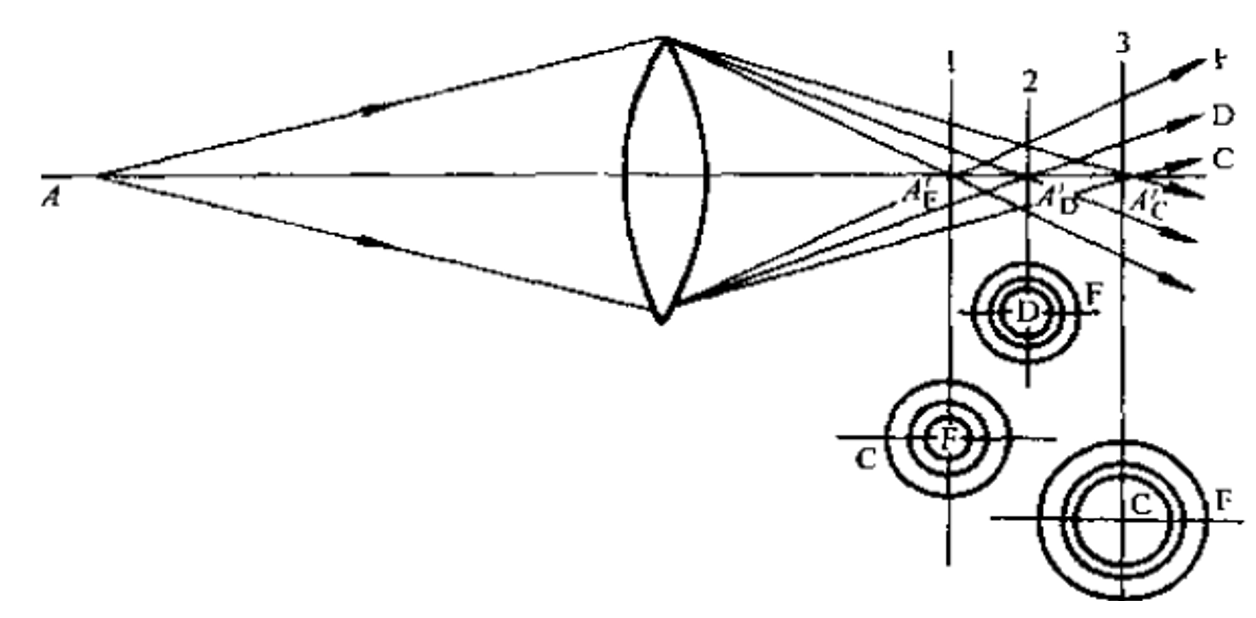
\includegraphics[width=0.85\textwidth]{graph2.png}
				\caption{位置色差}
				\label{fig:graph2}
			\end{figure}
		
		\item \textbf{慧差(Spherical Aberration)} :主要表现为在小视场和大孔径条件下产生的像差。慧差主要针对轴外光束,当光学系统不满足等晕条件时,轴外光束的对称性被破坏,导致成像光束与高斯像面相交成一个彗星状的弥散斑。孔径边缘上的光线在像面上的交点形成一个圆,距离孔径中心越近的圆周上的光线形成的交点圆越小,距离主光线和像面焦点越近。慧差可分为子午慧差和弧矢慧差,分别表示孔径边缘上、下光线和弧矢光线在像面上的交点与像面焦点的距离。慧差的存在会导致轴外像点成为彗星状的弥散斑,影响轴外像点的清晰度。
	\end{enumerate}

		\begin{figure}[htbp]
			\centering
			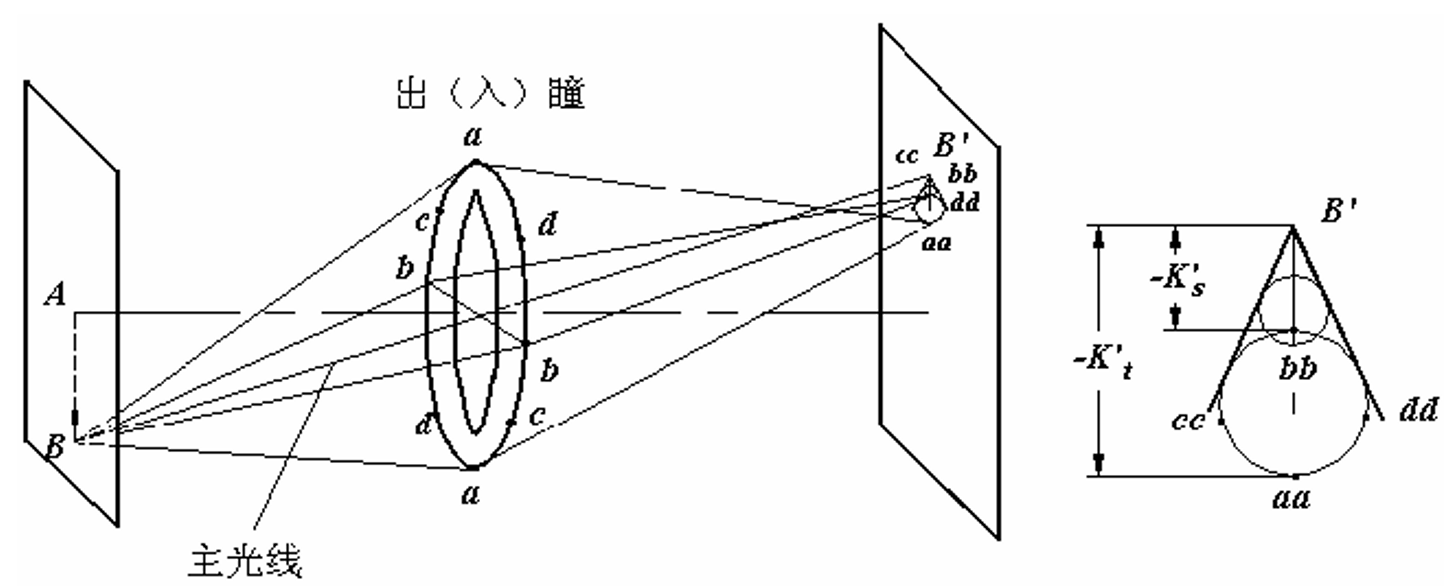
\includegraphics[width=0.85\textwidth]{graph1.png}
			\caption{慧差成像示意图和子午慧差、弧矢慧差}
			\label{fig:graph1}
		\end{figure}
	

\subsection{实验前思考题}
	\begin{question}
		慧差与孔径、视场的关系?
	\end{question}
		
		\begin{enumerate}
			\item \textbf{孔径对慧差的影响}:孔径越大,通过光学系统的光线范围越广,慧差产生的影响也就越显著。在大孔径条件下,光线在光学系统中的传播路径更加复杂,不同位置的光线会汇聚到不同的焦点上,导致成像质量下降,慧差效应更加明显。

			\item \textbf{视场对慧差的影响}:视场指的是在成像平面上能够接收光线的范围。在小视场条件下,成像平面上只有部分光线能够到达,此时慧差对成像的影响相对较小。然而,在大视场条件下,不同位置的光线经过光学系统后会形成不同位置的焦点,慧差会导致成像位置偏离预期位置,影响成像质量。
		\end{enumerate}
		
			
		
		
		
		
		

	\begin{question}
		产生色差原因?列举几种消色差的方法
	\end{question}

	产生色差的主要原因是介质对不同波长的光的折射率不同,导致不同波长的光线在经过光学系统后成像位置不同。具体来说,产生色差的原因包括:
	\begin{enumerate}
		\item \textbf{介质色散}:介质对不同波长的光的折射率不同,这种现象称为色散。在透镜或光学系统中,不同波长的光线经过折射后会有不同的折射角,导致不同波长的光线聚焦于不同位置。
		\item \textbf{透镜形状}:透镜的形状不同会导致不同波长的光线经过透镜后的光程不同,从而引起色差。例如,球面透镜的球差会导致不同波长的光线聚焦于不同位置。
		\item \textbf{玻璃材料}:不同的玻璃材料对不同波长的光的折射率不同,使用不同材料制作的透镜或光学元件会产生色差。
	\end{enumerate}
	
	几种消色差的方法包括:
	
	\begin{enumerate}
		\item \textbf{复合透镜设计}:使用多个透镜组合成复合透镜,利用不同透镜的特性来抵消色差。
		\item \textbf{使用折射率不同的玻璃材料}:选择折射率不同的玻璃材料组合制作透镜,使得不同波长的光线经过透镜后折射角相近,从而减小色差。
		\item \textbf{非球面透镜设计}:设计非球面透镜以校正球差和像差,可以减小色差。
		\item \textbf{色差补偿镜片}:在透镜组合中加入特殊设计的色差补偿镜片,用于校正不同波长的光线的色差。
		\item \textbf{光栅消色差}:使用光栅结构的光学元件,在不同波长的光线上产生不同的光程补偿,从而减小色差。
	\end{enumerate}

	
	
	
	


	\begin{question}
		针孔滤波的工作原理
	\end{question}

	针孔滤波是一种光学滤波方法,其工作原理基于衍射现象。当光线穿过一个非常小的孔径时,会发生衍射现象,即光线在经过孔径后会呈现出特定的衍射图样。针孔滤波利用这种衍射效应来控制光线的传播和成像。

	针孔滤波的工作原理如下:
	
	\begin{enumerate}
		\item \textbf{光线穿过孔径}:光线从光源处发出,经过一个非常小的孔径(针孔)后,会形成衍射图样。孔径的尺寸决定了通过的光线范围。
		
		\item \textbf{衍射效应}:光线通过孔径后,会在成像平面上形成衍射图样,这是由于光波在经过孔径时会发生弯曲和相互干涉的结果。衍射图样的形状和大小取决于孔径的尺寸和光波的波长。
		
		\item \textbf{滤波效果}:针孔滤波器根据衍射图样的特性来选择通过的光线。通常,衍射图样中心的光强最强,周围逐渐减弱,因此可以通过调整孔径的尺寸和光源与成像平面的距离来控制通过的光线,实现对光的滤波。
		
		
	\end{enumerate}

	应用:针孔滤波器常用于显微镜等光学系统中,用于控制成像的分辨率和对比度。通过调整针孔的尺寸和位置,可以改变成像的清晰度和细节表现。



\clearpage
\begin{table}
	\renewcommand\arraystretch{1.7}
	\centering
	\begin{tabularx}{\textwidth}{|X|X|X|X|}
	\hline
	专业:& 物理学 &年级:& 2022级 \\
	\hline
	姓名:& 戴鹏辉 & 学号:& 22344016 \\
	\hline
	室温:&  & 实验地点: &  \\
	\hline
	学生签名:& & 评分: &\\
	\hline
	日期:&  & 教师签名:&\\
	\hline
	\end{tabularx}
\end{table}

\section{光学像差实验I \quad\heiti 实验记录}
\subsection{实验内容、步骤、结果及讨论}\textcolor{ForestGreen}{(按照实验顺序依次}\textcolor{red}{简要记录}\textcolor{ForestGreen}{实验内容及步骤,)(空间不够,可自行加页)}\\
\textcolor{red}{
(注意: \\
除了记录实验内容、步骤、参数外,还应记录:\\
按比例绘制操作中实际摆放的实验光路(各元件间距离可通过直尺测量)\\
记录光路中物光和参考光的光程差\\
记录物光和参考光光强比\\
记录是否可观察到再现图像\\
)
}


		

%\subsection{实验数据记录}



%\subsection{原始数据记录}

\clearpage

\newpage

\null

\newpage

\null






\newpage

\subsection{实验过程中遇到的问题记录}

	\begin{enumerate}
		\item 
		\item 
		\item 
	\end{enumerate}
\null




% \begin{table}
% 	\renewcommand\arraystretch{1.7}
% 	\begin{tabularx}{\textwidth}{|X|X|X|X|}
% 	\hline

% 	专业:& 物理学 &年级:& 2022级\\
% 	\hline
% 	姓名: & 戴鹏辉 & 学号:& 22344016\\
% 	\hline
%     日期:& 2024/xx/xx & 评分: &\\
% 	\hline
% 	\end{tabularx}
% \end{table}

% \section{全息照相实验 \quad\heiti 分析与讨论}

% \subsection{实验数据分析}

% 	\subsubsection{实验一 测量光栅常数}
	
		
% 	\subsubsection{实验二 测定未知光波波长及角色散率D}
			

			
% \subsection{实验后思考题}



% \begin{question}
% 	检索文献,列举三种测量光波波长的方法,给出参考文献列表。%\lipsum[20]
% \end{question}
	

	



\end{document}
